\documentclass[]{article}

\usepackage{graphicx}
\graphicspath{ {Images/} }
\usepackage{titlesec}
\usepackage{wrapfig}

\titleformat{\section}
  {\normalfont\Large\bfseries}{\thesection}{1em}{}[{\titlerule[0.8pt]}]

\begin{document}

\title{IACS-Copmutes! 2016 Teaching Assistants}

\section*{Joel Anderson} {
\begin{wrapfigure}{R}{0.2\textwidth}
\begin{centering}
    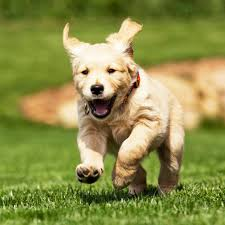
\includegraphics[width=0.2\textwidth]{puppy.jpeg}
\end{centering}
\end{wrapfigure}
Joel's paragraph. }
\vspace{1.25 in}

\section*{Connor Behan} {
\begin{wrapfigure}{R}{0.2\textwidth}
\begin{centering}
    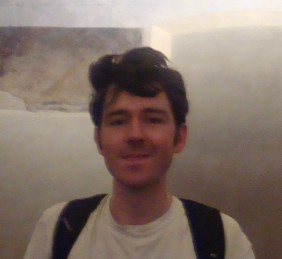
\includegraphics[width=0.2\textwidth]{connor.jpg}
\end{centering}
\end{wrapfigure}
I'm a grad student in Stony Brook's Department of Physics and Astronomy with a hobby of testing patches for a number of random Linux programs. Working with Leonardo Rastelli, I am studying the interplay between quantized fields and various phase transitions in matter, \textit{e.g.} solid to liquid or paramagnetic to ferromagnetic. A program I developed to make this task easier is PyCFTBoot, written in Python. }
\vspace{1.25 in}

\section*{Panu Sam-Ang} {
\begin{wrapfigure}{R}{0.2\textwidth}
\begin{centering}
    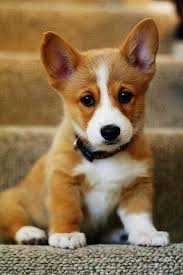
\includegraphics[width=0.2\textwidth]{puppy3.jpeg}
\end{centering}
\end{wrapfigure}
Panu's paragraph. }
\vspace{1.2 in}

\section*{Bryan Sundahl} 
\begin{wrapfigure}{R}{0.2\textwidth}
\begin{centering}
    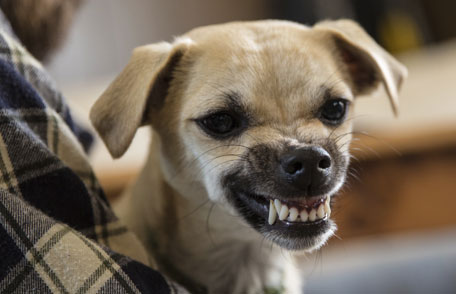
\includegraphics[width=0.193\textwidth]{grumpy.jpeg}
\end{centering}
\end{wrapfigure}
I'm a graduate student in Applied Math and Statistics here at Stony Brook University, working in the lab of Robert Harrison. My research involves creating software to model the response of molecules to external perturbations (e.g. lasers).  Python is the main tool in my analysis of these models. 

\end{document}
